\section{Memoria del proyecto}
\label{memoria}
\emph{En este capítulo se describirá cómo se ha llevado a cabo el proyecto, qué cambios se han hecho respecto a la versión inicial, imprevistos surgidos, etc}

A continuación se describen los objetivos principales de cada uno de los equipos de trabajo así como un pequeño resumen de cómo se ha desarrollado el trabajo de cada equipo en esta primera iteración. En el resto de la sección se describe detalladamente todo el desarrollo del proyecto.\\
\subsubsection*{BackEnd}
El objetivo del equipo backend era desarrollar un paquete de java que representase la lógica del juego del guiñote, al mismo tiempo que desarrollaba gran parte de la página web dinámica del proyecto. Sin embargo a mitad de desarrollo el trabajo se centró en acabar la parte de la lógica del juego en 3 semanas. Dicho objetivo no se ha cumplido completamente dado que el desarrollo de este modulo se alargó media semana más. Como consecuencia la web dinámica arrastra un leve retraso que deberá ser compensado en la segunda iteración. A pesar de dichas dificultades el equipo ha trabajado mucho para conseguir una primera versión funcional antes de la primera iteración.

\subsubsection*{Base de datos}
Los dos principales objetivos del equipo de bases de datos eran por una parte diseñar e implementar la base de datos para el sistema(esquema conceptual, lógico y físico) y por otra desarrollar la capa de acceso a datos proporcionando una interfaz para el backend. Los dos objetivos se han cumplido prácticamente en su totalidad, con excepción de la parte de acceso a datos relacionada con los torneos, que no ha sido posible terminar de implementar y será finalizada en la segunda iteración. Exceptuando las pequeñas dificultades iniciales relacionadas con un tardío diseño de la interfaz de acceso a datos, tanto la comunicación entre los miembros del equipo como con el resto de equipos relacionados con el acceso a los datos se ha desarrollado sin problemas.

\subsection{Inicio del proyecto}
\label{Inicio del proyecto}
\emph{Describir cómo transcurrió esta fase del proyecto, especialmente los resultados de llevar a cabo los procesos descritos en la sección Procesos de inicio del proyecto.}
\subsubsection*{BackEnd}
Durante la primera semana el equipo adquirió y configuró el software de desarrollo intellij IDEA. Tras una primera toma de contacto comenzó el trabajo. Sin embargo, a lo largo de la primera iteración el equipo se ha encontrado con diferentes problemas de integración debido a la inexperiencia del IDE. Por lo tanto en futuros proyectos sería recomendable incluir en formación la adquisición de experiencia con los IDE's.
\subsubsection*{Base de datos}
En el inicio del proyecto el equipo realizó la configuración de la base de datos en AWS, utilizando Amazon Aurora sobre MySQL como se había decidido. Las principales características de la base de datos utilizada para el proyecto se detallan a continuación:

\begin{lstlisting}
Aurora compatible mysql 5.7.12

db.t2.small - 1 CPU, 2 GIB RAM

Instance identifier: sotayrey-aurora

DB cluster identifier: sotayrey-cluster

Database name: sotayrey\_db

Backup every 30 days
\end{lstlisting}

Las características seleccionadas se deben al requerimiento de utilizar solamente aquellos recursos disponibles para la versión gratuita de estudiantes, que es con la que se está trabajando. Además, el servidor de base de datos se ha configurado de forma que se puede acceder desde el exterior para hacer más fácil el acceso durante el desarrollo de la base de datos, pero este será deshabilitado una vez el sistema esté desplegado, por razones de seguridad.\\

En cuanto a formación, el equipo de bases de datos se formó en el funcionamiento de la api JDBC, así como en la utilización de pools de conexiones con c3p0. Al contrario de lo que se había establecido en los procesos de inicio del proyecto (sección \ref{inicio}), el equipo no se formó en lo que respecta a HTML/CSS y JSP, porque no lo requería para sus competencias en la primera iteración.
\subsection{Ejecución y control del proyecto}
\label{Ejecucion y control del proyecto}
\emph{
Describir cómo transcurrió esta fase del proyecto, especialmente los resultados de llevar a cabo los procesos descritos en la sección Procesos de ejecución y control del proyecto y en la sección Procesos técnicos. No olvidar:
Cómo se ha realizado el reparto de trabajo entre miembros del equipo. Cómo ha transcurrido la comunicación interna. 
Cómo se ha medido el progreso del proyecto. Cómo se sabía el trabajo realizado, el trabajo pendiente y lo que estaba haciendo cada persona.
Los ajustes realizados cuando se detectaron divergencias frente al calendario inicial (ajustes en el trabajo y/o ajustes en el calendario). Si se han identificado las causas de estas divergencias, explicarlas.
Adecuación de las herramientas y tecnologías empleadas. Si ha habido que cambiar alguna decisión de diseño o de tecnología, y por qué.
Funcionamiento de los procesos de control de versiones del código, construcción y despliegue. ¿Ha habido problemas con las integraciones? ¿Problemas con los despliegues? ¿Se han perdido cosas por errores humanos? ¿Cómo se han abordado estas tareas?
Pruebas del software. ¿Se han podido cumplir las ideas que se tenían al respecto?}
\subsubsection{Reparto del trabajo}
En un primer momento, el reparto de trabajo fue definido únicamente en relación a los equipos creados, como se detalla en la sección \ref{repartotrabajo}. Sin embargo, se detectó que este reparto, aunque necesario, era demasiado genérico y no permitía medir el progreso de forma clara. Por ello se decidió que dentro de cada equipo de trabajo se llevaría a cabo una división del trabajo en tareas o paquetes de trabajo, siguiendo la Estructura de Descomposición del Trabajo (WBS \cite{edt}). Cada paquete de trabajo corresponde a una tarea específica y claramente delimitada, como puede ser el desarrollo de una clase, y especifica un único responsable de este (no significa que sea la única persona que trabaje en él pero sí la responsable de su desarrollo). Para el control del progreso en relación a esta división del trabajo se ha utilizado el apartado Projects de GitHub, en el que cada paquete se marca con un tick cuando está finalizado y depurado.
\begin{figure}[H]
		\hspace{-2cm}
		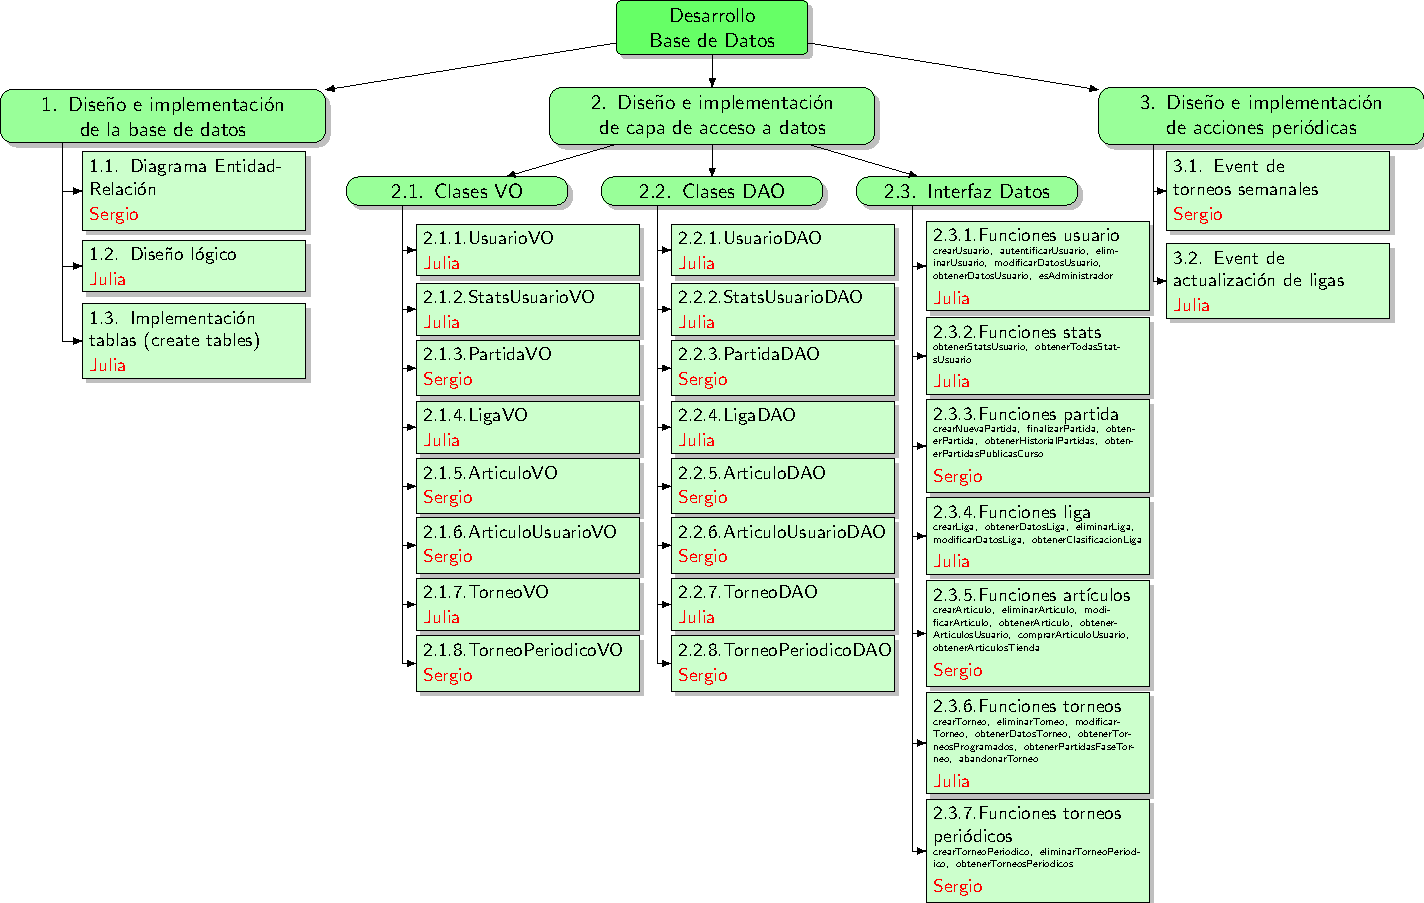
\includegraphics[scale=0.8]{figuras/edtBasesDatos.pdf}
		\caption{Diagrama de Paquetes de Trabajo Bases de Datos}
	\end{figure}

\begin{figure}[H]
		\centering
		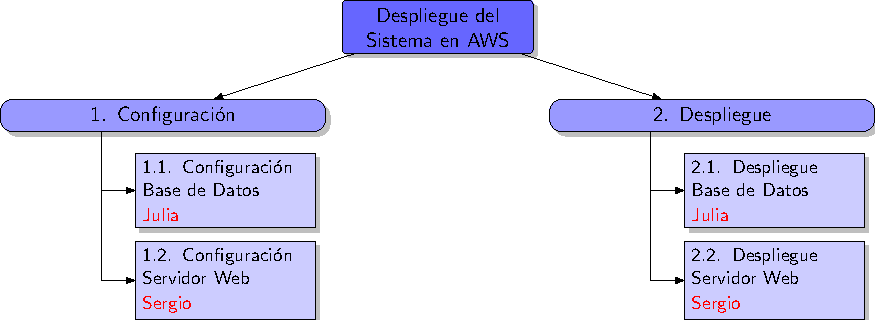
\includegraphics[scale=0.8]{figuras/edtDespliegue.pdf}
		\caption{Diagrama de Paquetes de Trabajo Despliegue}
	\end{figure}

Es importante añadir que el trabajo de integración de los diferentes paquetes de trabajo no está reflejado en estos diagramas pero también ha sido necesario repartirlo y realizarlo.
\subsubsection{Comunicación interna}
\subsubsection{Adecuación a las herramientas y tecnologías}
\subsubsection{Control de versiones}
\subsubsection{Integración y despliegue}
En cuanto a la integración entre el acceso a datos y el backend, se detectó un claro problema de comunicación entre los grupos a mitad del desarrollo debido a que no existía una interfaz definida de forma precisa desde un primer momento. Únicamente se había comentado una interfaz ambigua que diferentes partes entendían de forma distinta, y que además, sin las definiciones concretas de las funciones, impedía llevar a cabo el desarrollo en paralelo. Cuando se detectó el problema, hubo una reunión entre ambos grupos para definir esta interfaz de acceso a los datos y fue solucionado el problema. Gracias a este incidente se ha aprendido la importancia del desarrollo de interfaces entre los distintos componentes de los sistemas.
El despliegue del servidor de bases de datos se realizó en AWS sin mayores problemas. En cuanto al despliegue del servidor web,...TODO
\subsubsection{Pruebas del software}
\subsubsection*{Bases datos}
La base de datos implementada en MySQL fue probada mediante la inserción de datos falsos de ejemplo, y la realización de consultas sencillas sobre ella, que garantizan el correcto funcionamiento. La interfaz de acceso a datos ha sido probada mediante pruebas unitarias. Se desarrolló un programa de pruebas al final del desarrollo de cada clase DAO, probando función a función sobre los datos de ejemplo introducidos, y solucionando errores de implementación.

\subsubsection{Progreso}
\subsubsection*{Divergencias frente a la planificación inicial}
\subsubsection*{Bases datos}
En general se ha cumplido el diagrama de Gantt establecido, exceptuando la implementación del acceso a datos relacionado con los torneos, que estaba planificado para la primera iteración y se debe alargar a la segunda, sin suponer ningún problema de dependencias con el resto de componentes del sistema. También se puede comentar que, en lo que respecta al diseño de la base de datos, se requirió algo menos tiempo del estimado (se finalizó con una semana de antelación), mientras que el diseño del acceso a datos requirió más tiempo del estimado por lo que fueron compensados, cumpliendo bastante bien la planificación inicial.
